\documentclass[oneside,11pt,letter]{article}

% General include (DO NOT MODIFY)
\usepackage{amsmath,graphicx,cite,latexsym,color, amssymb,ifthen,verbatim}

\usepackage{listings, url}
\definecolor{mygreen}{rgb}{0,0.6,0}
\definecolor{mygray}{rgb}{0.5,0.5,0.5}
\definecolor{mymauve}{rgb}{0.58,0,0.82}

\lstset{ %
  backgroundcolor=\color{white},   % choose the background color
  basicstyle=\footnotesize,        % size of fonts used for the code
  breaklines=true,                 % automatic line breaking only at whitespace
  captionpos=b,                    % sets the caption-position to bottom
  commentstyle=\color{mygreen},    % comment style
  escapeinside={\%*}{*)},          % if you want to add LaTeX within your code
  keywordstyle=\color{blue},       % keyword style
  stringstyle=\color{mymauve},     % string literal style
}
\lstset{basicstyle=\small\ttfamily,breaklines=true}

%--------------- Various Style Declarations ----------------------------
\textheight 9in
\topmargin 0in
\headheight 0in
\headsep 0in
\textwidth 6.5in
\oddsidemargin 0in
\evensidemargin 0in
\footskip 0.2in
\parskip 5pt
\parindent 0pt
\topsep 2pt
\partopsep 0pt
\itemsep 0pt
\pagenumbering{arabic}

\definecolor{shade}{gray}{0.85}


\newcommand{\solpagesize}%
{\ifthenelse{\equal{\type}{solutions}}{
\textheight9in
\textwidth6.5in
\oddsidemargin0in
\evensidemargin0in
\topmargin-0.75in
\topskip0in
\footskip0.70in
\pagestyle{empty}
\parskip 5pt
\parindent 0pt
}{}}

\newcommand{\bookletskip}[1] %
{\ifthenelse{\equal{\type}{booklet}}{\vspace{#1 in}}
}

\newcommand{\bookletpage} %
{\ifthenelse{\equal{\type}{booklet}}{\newpage}{}
}

\newcommand{\inbooklet}[1]{\ifthenelse{\equal{\type}{booklet}}{{#1}}}


%%%%%%%%%%%%%%%%%%%%%%%%%%%%%%%%%%%%%%%
% Here are the new definitions of the commands \problem (for main
% text of problem), \problempart (for parts (a), (b) etc of the problem
% and \solution (for text of the solution).  The usage is as follows.
%
%    \begin{enumerate}
%    \problem{label}{main text of first problem}
%    \begin{enumerate}
%    \problempart{text of part(a) of first problem}
%
%    \solution{text of solution to part(a)}
%    \problempart{\text of part(b)}
%
%    \solution{text of solution to part (b)}
%
% ..... and so on for succeeding parts
%
%    \end{enumerate}
%
%    \problem{label}{main text of second problem}
%    \begin{enumerate}
%    \problempart{text of part(a)}
%
%    \solution{text of solution to part(a)}
%    \problempart{\text of part(b)}
%
%    \solution{text of solution to part (b)}
%    \end{enumerate}
%    ........ and so on for other problems
%    \end{enumerate}
%
% Please note that there needs to be a blank line separating
% a problempart command and the succeeding solution command;
% else the problem part and the solution are typeset as one
% paragraph when we are printing both the problem and its
% solution.  However, it is OK if a problempart follows a
% previous solution without an intervening blank line.  Some day I will
% waste some time figuring out a way around this problem

\newcommand{\problem}[2]%
{\item\label{#1}%
\ifthenelse{\(\equal{\type}{problems}\)\or\(\equal{\type}{both}\)}%
 {{\bf[#1]\\}#2}{{\bf[#1]}}}
 % The problem name always prints on the first line (in boldface
 % and inside square brackets.  The problem text prints on
 % succeeding lines if we are printing problems only, or problems
 % and solutions both

  \newcommand{\problempart}[1]%
{\item{\ifthenelse{\(\equal{\type}{problems}\)\or\(\equal{\type}{both}\)}%
 {#1}{}}}
 % The tag ((a), or (b) or (c) etc.) of the text of the part of the problem
 % prints in the margin, and is followed by the text of the problem beginning
 % on the same line if we are printing problems only or problems and
 % solutions both

 \newcommand{\solution}[1]%
{\ifthenelse{\equal{\type}{both}}{{\bf{Solution:\ }}{#1}}%
 {\ifthenelse{\(\equal{\type}{solutions}\)}%
 {#1}{}}}
 % This command does not generate a tag ((a), or (b) or (c) etc.)
 % for the text, but uses the tag generated by the previous 
 % problempart or examproblempart command.  If only the solutions 
 % are being printed, then the text
 % of the solution is printed beginning on the same line as the tag.
 % If both problems and solutions are being printed, then "Solution:"
 % is printed in boldface followed by the text of the solution.

  %%%%%%%%%%%%%%%%%%%%%%%%%%%%%%%%%%%%%%%%%
  
  
 \newcommand{\examproblem}[2]%
{\item {\ifthenelse{\equal{\type}{solutions}}{}{{\bf [#1 points]} #2}}}
% The first argument is an integer specifying the number of points.  The
% first argument (followed by the word "points") is printed inside square
% brackets in boldface.  The second argument is the text of the problem
% itself.


\newcommand{\examproblempart}[1]%
{\item{\ifthenelse{\(\equal{\type}{problems}\)\or\(\equal{\type}{both}\)\or\(\equal{\type}{booklet}\)}%
 {#1}{}}}
 % The tag ((a), or (b) or (c) etc.) of the text of the part of the problem
 % prints in the margin, and is followed by the text of the problem beginning
 % on the same line if we are printing problems only or problems and
 % solutions both

%%%%%%%  ENTER SOME PROBLEM SET SPECIFIC STUFF HERE  %%%%



%%%%%%%%%%%%%%%%%%%%%%
%CHANGE
%.   to booklet to print the problems only
%
%    to both to print problems and solutions
%%%%%%%%%%%%%%%%%%%%%%

\newcommand{\type}{booklet}
% \newcommand{\type}{both}

% Custom adjustments (CHANGE THIS FILE FOR ADDITIONAL ADJUSTMENTS)
\usepackage{tikz}
\newcommand{\cN}{{\cal N}}

\DeclareMathOperator*{\argmin}{\arg\!\min}
\newcommand{\norm}[1]{\left\lVert#1\right\rVert}

%************************************************************************
%                                                                       *
%            End of preamble and beginning of text.                     *
%                                                                       *
%************************************************************************

\begin{document}
%------------------------- Title Page ----------------------------------
\thispagestyle{empty}
\baselineskip2.5ex
{\bf University of Illinois}
\hfill
Spring 2018

{\Large
\begin{center}
{\sf CS\,446: Machine Learning}\\ Homework 9\\
\end{center}
}
{\large
\begin{center}
{\color{red}Due on Tuesday, April 3, 2018, 11:59 a.m. Central Time}
\end{center}
}

\ifthenelse{\equal{\type}{booklet}}{}{}

\begin{enumerate}

%%%%%%%%%%%%%%%%%%%%%%%%%%%%%%%%%%%%%%
%%%%%  BEGINNING OF PROBLEMS LIST

% !TEX root = exam.tex
\ifthenelse{\equal{\type}{booklet}}{
\newcommand{\GMMkMeansStudSolA}{
%%%%%%%%%%%%%%%%%%%%%%%%%%%%%%%%%%%%
%%
%%.   YOUR SOLUTION FOR PROBLEM A BELOW THIS COMMENT
%%
%%%%%%%%%%%%%%%%%%%%%%%%%%%%%%%%%%%%
Unsupervised. It doesn't use any kind of label.
}

\newcommand{\GMMkMeansStudSolB}{
%%%%%%%%%%%%%%%%%%%%%%%%%%%%%%%%%%%%
%%
%%.   YOUR SOLUTION FOR PROBLEM A BELOW THIS COMMENT
%%
%%%%%%%%%%%%%%%%%%%%%%%%%%%%%%%%%%%%
By adding a constraint on $r_{ik}$. We would want $r_{ik}$ to be 1 for one, and only one, $k$ for each $i$. So, our constraints can be written as:
\[ r_{ik} \in \{0, 1\} \hspace{0.3cm} \forall i \in \{1, 2, \cdots, D \}, \forall r \in \{1, 2, \cdots, K \} \eqno{(1)}\]
\[ \sum_{k=1}^K r_{ik} = 1 \hspace{0.3cm} \forall i \in \{1, 2, \cdots, D \} \eqno{(2)} \]

Additional to those constraints we could also specify a constraint to ensure the active $k$ is the one corresponding to the closest center:
\[ r_{ik} = \delta\left( k = \argmin_j ||x_i - \mu_j ||^2 \right) \]
}

\newcommand{\GMMkMeansStudSolC}{
%%%%%%%%%%%%%%%%%%%%%%%%%%%%%%%%%%%%
%%
%%.   YOUR SOLUTION FOR PROBLEM A BELOW THIS COMMENT
%%
%%%%%%%%%%%%%%%%%%%%%%%%%%%%%%%%%%%%
Replace the integrity constraint $r_{ik} \in \{0, 1\}$ with $r_{ik} \in [0, 1]$ and ignore the $\delta$ function.
}

\newcommand{\GMMkMeansStudSolD}{
%%%%%%%%%%%%%%%%%%%%%%%%%%%%%%%%%%%%
%%
%%.   YOUR SOLUTION FOR PROBLEM A BELOW THIS COMMENT
%%
%%%%%%%%%%%%%%%%%%%%%%%%%%%%%%%%%%%%
Using the Elbow method\footnote{\url{https://en.wikipedia.org/wiki/Elbow_method_(clustering)}} we can say that $k = 5$ is the best choice because after that the cost decrease is too small.
}

\newcommand{\GMMkMeansStudSolE}{
%%%%%%%%%%%%%%%%%%%%%%%%%%%%%%%%%%%%
%%
%%.   YOUR SOLUTION FOR PROBLEM A BELOW THIS COMMENT
%%
%%%%%%%%%%%%%%%%%%%%%%%%%%%%%%%%%%%%
The basic $k$-means, using Euclidean distance, is certainly not enough to cluster the provided data. The reason for this is that $k$-means tries to find non-overlapping spherical clusters. This is a consequence of using Euclidean distance and not of the $k$-means algorithm per se.  But $k$-means can be used with a whole family of distance functions. There are distance functions that are kernel based that can effectively identify clusters in this data. A Gaussian Kernel based distance is one of them \footnote{\url{https://sites.google.com/site/dataclusteringalgorithms/kernel-k-means-clustering-algorithm}}, this is sometimes referred as Spectral clustering.
}

%\newcommand{\GMMkMeansStudSolF}{
%%%%%%%%%%%%%%%%%%%%%%%%%%%%%%%%%%%%%
%%%
%%%.   YOUR SOLUTION FOR PROBLEM A BELOW THIS COMMENT
%%%
%%%%%%%%%%%%%%%%%%%%%%%%%%%%%%%%%%%%%
%}
 %The students have to fill this file to print the solution
}{
\input{GMMkMeans_OurSolution} %This file will not be provided to students since it contains the solution
}

% Problem Explanation:
% - first argument is the number of points
% - second argument is the title and the text
\examproblem{10}{K-Means\\}


%%%%%%%%%%%%%%%%%%%%%%%%%%%%%%%%%%%%%%
%%%%%  BEGINNING OF SUBPROBLEMS LIST

\begin{enumerate}

 % Subproblem description
\examproblempart{Mention if K-Means is a supervised or an un-supervised method.
 \\}

\bookletskip{0.0}   %in inches

% Solution box
 \framebox[14.7cm][l]{
 \begin{minipage}[b]{14.7cm}
 \inbooklet{Your answer: \GMMkMeansStudSolA}
  
 \solution{\GMMkMeansSolA}
 \end{minipage}
 }
 
  % Subproblem description
\examproblempart{Assume that you are trying to cluster data points $x_{i}$  for $ i \in \{1,2 \dots D\}$ into K clusters each with center $\mu_{k}$  where $ k \in \{1,2, \dots K \}$. The objective function for doing this clustering involves minimizig the euclidean distance between the points and the cluster centers. It is given by  \begin{equation*}
\min\limits_{\mu} \min\limits_{r}\sum\limits_{i \in D} \sum\limits_{k =1}^{K} \frac{1}{2} r_{ik} ||x_{i} -\mu_{k}||_{2}^{2} \\
 \end{equation*} \\ How do you ensure hard assignemnt of one data point to one and only one cluster at a given time? Note: By hard assignment we mean that your are 100 \% sure that a point either belongs or not belongs to a cluster.\\}

\bookletskip{0.0}   %in inches

% Solution box
 \framebox[14.7cm][l]{
 \begin{minipage}[b]{14.7cm}
 \inbooklet{Your answer: \GMMkMeansStudSolB}
  
 \solution{\GMMkMeansSolB }
 \end{minipage}
 }
 
% Subproblem description
\examproblempart{What changes must you do in your answer of part b, to make the hard assingment into a soft assignment? Note: By soft assignment we mean that your are  sure that a point either belongs or not belongs to a cluster with some probability.\\}

\bookletskip{0.0}   %in inches

% Solution box
 \framebox[14.7cm][l]{
 \begin{minipage}[b]{14.7cm}
 \inbooklet{Your answer: \GMMkMeansStudSolC}
  
 \solution{\GMMkMeansSolC}
 \end{minipage}
 }
 
 % Subproblem description
 \examproblempart{Looking at the following plot, what is the best choice for number of clusters?}
  \begin{center}
 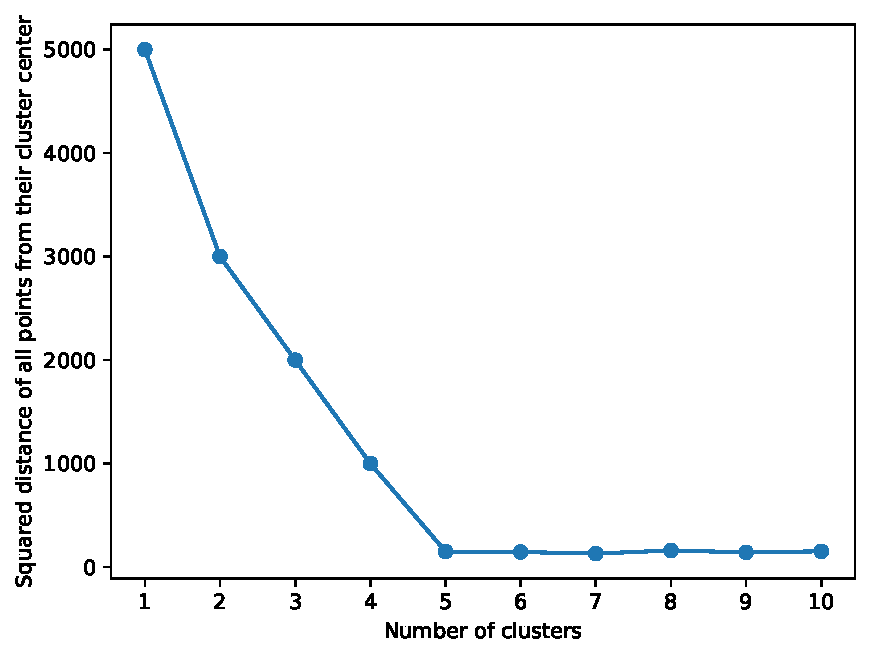
\includegraphics[width=8cm]{fig/cluster.pdf}
 \end{center}
\bookletskip{0.0}   %in inches

% Solution box
 \framebox[14.7cm][l]{
 \begin{minipage}[b]{14.7cm}
 \inbooklet{Your answer: \GMMkMeansStudSolD}
  
 \solution{\GMMkMeansSolD}
 \end{minipage}
 }

% Subproblem description
 \examproblempart{Would K-Means be an effecient algorithm to cluster the following data? Explain your answer in a couple of lines.}
  \begin{center}
 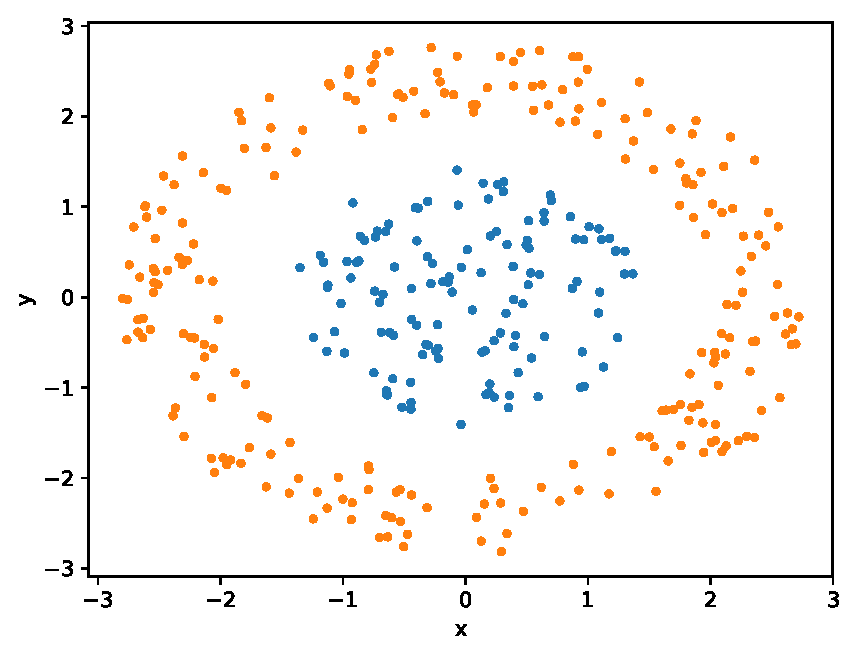
\includegraphics[width=8cm]{fig/concentric.pdf}
 \end{center}
\bookletskip{0.0}   %in inches

% Solution box
 \framebox[14.7cm][l]{
 \begin{minipage}[b]{14.7cm}
 \inbooklet{Your answer: \GMMkMeansStudSolE}
  
 \solution{\GMMkMeansSolE}
 \end{minipage}
 }
 
 %}
 
  %%%%%%%%%%%% END OF SUBPROBLEMS LIST
  
 \end{enumerate}
\bookletpage

Lets take the objective function from c)
\[
\sum_{k=1}^K z_{ik} \left(
		\log \pi_k + \log \mathcal{N}\left(x_i | \mu_k, \sigma_k \right)
	\right)
\]
and lets also remember the explicit constraint that $\sum_k \pi_k = 1$. Note that we need to sum over the entire data set so we then can write the dual of the objective function:
\begin{align*}
F &= \sum_{i=1}^N \left( \sum_{k=1}^K z_{ik} \left(
		\log \pi_k + \log \mathcal{N}\left(x_i | \mu_k, \sigma_k \right)
	\right) \right) + \lambda \left( \sum_k \pi_k - 1 \right)\\
&= \sum_{i=1}^N \sum_{k=1}^K z_{ik}\log \pi_k +
	\sum_{i=1}^N \sum_{k=1}^K z_{ik} \log \mathcal{N}\left(x_i | \mu_k, \sigma_k \right)
	 + \lambda \left( \sum_k \pi_k - 1 \right)
\end{align*}
Now lets take the derivative with respect to the variables we want to update on each step and set it to zero:

a) For $\pi_k$ (refers to $\pi_k^{(t+1)}$):
\begin{align*}
\frac{\partial F}{\partial \pi_k} &= \sum_{i=1}^N z_{ik} \frac{1}{\pi_k} + 0 + \lambda = 0 
\iff \pi_k = \frac{\sum_{i=1}^N z_{ik}}{-\lambda}
\end{align*}
By using the constraint:
\begin{align*}
1 = \sum_{k=1}^K \pi_k &= \sum_{k=1}^K \frac{\sum_{i=1}^N z_{ik}}{-\lambda}\\
&= \frac{\sum_{i=1}^N \sum_{k=1}^K z_{ik}}{-\lambda}\\
&= \frac{\sum_{i=1}^N 1}{-\lambda}\\
&= \frac{N}{-\lambda}\\
\rightarrow \lambda &= -N
\end{align*}
Then
\begin{align*}
0 = \frac{\partial F}{\partial \pi_k}  &= \sum_{i=1}^N z_{ik} \frac{1}{\pi_k} + \lambda = \sum_{i=1}^N z_{ik} \frac{1}{\pi_k} - N\\
\rightarrow \pi_k^{(t+1)} &= \frac{1}{N}\sum_{i=1}^N z_{ik}
\end{align*}

\pagebreak

\newcommand{\gaussian}{
	\left(2\pi \sigma_k^2\right)^{-\frac{1}{2}} \exp \left(
			-\frac{1}{2\sigma_k^2} \left( x_i - \mu_k \right)^2
		\right)
}

b) For $\mu_k$:\\
\begin{align*}
0 &= \frac{\partial F}{\partial \mu_k}\\
&=  \frac{\partial}{\partial \mu_k} \left( \sum_{i=1}^N \sum_{k=1}^K z_{ik}\log \pi_k +
	\sum_{i=1}^N \sum_{k=1}^K z_{ik} \log \mathcal{N}\left(x_i | \mu_k, \sigma_k \right)
	 + \lambda \left( \sum_k \pi_k - 1 \right) \right)\\
&= \frac{\partial}{\partial \mu_k} \left( 
	\sum_{i=1}^N \sum_{k=1}^K z_{ik} \log \mathcal{N}\left(x_i | \mu_k, \sigma_k \right)
	 + \lambda \left( \sum_k \pi_k - 1 \right) \right)\\
&= \frac{\partial}{\partial \mu_k}
	\sum_{i=1}^N z_{ik} \log \mathcal{N}\left(x_i | \mu_k, \sigma_k \right)\\
&=  \frac{\partial}{\partial \mu_k}
	\sum_{i=1}^N z_{ik} \log \gaussian\\
&=  \frac{\partial}{\partial \mu_k} \left(
	\sum_{i=1}^N z_{ik} \log \left(2\pi \sigma_k^2\right)^{-\frac{1}{2}} +
	\sum_{i=1}^N z_{ik}  \log \exp \left(
			-\frac{1}{2\sigma_k^2} \left( x_i - \mu_k \right)^2
		\right)
\right)\\
&=  \frac{\partial}{\partial \mu_k} \left(
	-\sum_{i=1}^N z_{ik} \log \left((2\pi)^{\frac{1}{2}} \sigma_k\right) +
	\sum_{i=1}^N z_{ik}  \left(
			-\frac{1}{2\sigma_k^2} \left( x_i - \mu_k \right)^2
		\right)
\right)\\
&=  \frac{\partial}{\partial \mu_k} \left(
	\sum_{i=1}^N z_{ik}  \left(
			-\frac{1}{2\sigma_k^2} \left( x_i - \mu_k \right)^2
		\right)
\right)\\
&= \sum_{i=1}^N z_{ik}  \left(
	\frac{1}{2\sigma_k^2} \left( x_i - \mu_k \right)
\right)\\
& \rightarrow \sum_{i=1}^N z_{ik}  \left( x_i - \mu_k \right) = 0\\
& \rightarrow \sum_{i=1}^N z_{ik} x_i = \sum_{i=1}^N z_{ik} \mu_k\\
& \rightarrow \mu_k = \frac{\sum_{i=1}^N z_{ik} x_i}{\sum_{i=1}^N z_{ik}}\\
& \rightarrow \mu_k =  \frac{\sum_{i=1}^N z_{ik} x_i}{N \pi_k^{(t+1)}} = \mu_k^{(t+1)}\\
\end{align*}

\pagebreak

c) For $\sigma_k$:\\
Reusing some derivations from b)
\begin{align*}
0 &= \frac{\partial}{\partial \sigma_k} \left(
	-\sum_{i=1}^N z_{ik} \log \left((2\pi)^{\frac{1}{2}} \sigma_k\right) +
	\sum_{i=1}^N z_{ik}  \left(
			-\frac{1}{2\sigma_k^2} \left( x_i - \mu_k \right)^2
		\right)
\right)\\
&= \frac{\partial}{\partial \sigma_k} \left(
	-\sum_{i=1}^N z_{ik} \log  \sigma_k +
	\sum_{i=1}^N z_{ik}  \left(
			-\frac{1}{2\sigma_k^2} \left( x_i - \mu_k \right)^2
		\right)
\right)\\
&= -\frac{1}{\sigma_k}\sum_{i=1}^N z_{ik} + \frac{1}{\sigma_k^3}\sum_{i=1}^N z_{ik} \left( x_i - \mu_k \right)^2
\end{align*}
Multiplying by $\sigma_k^3$ on both sides
\begin{align*}
0 &= -\sigma_k^2 \sum_{i=1}^N z_{ik} + \sum_{i=1}^N z_{ik} \left( x_i - \mu_k \right)^2\\
\sigma_k^2 \sum_{i=1}^N z_{ik} &= \sum_{i=1}^N z_{ik} \left( x_i - \mu_k \right)^2\\
\sigma_k^2 &= \frac{\sum_{i=1}^N z_{ik} \left( x_i - \mu_k \right)^2}{\sum_{i=1}^N z_{ik}}\\
\sigma_k^2 &= \frac{\sum_{i=1}^N z_{ik} \left( x_i - \mu_k \right)^2}{N\pi_k^{(t+1)}} = 
	\frac{\sum_{i=1}^N z_{ik} \left( x_i - \mu_k^{(t+1)} \right)^2}{N\pi_k^{(t+1)}}
\end{align*}

%%%%%%%%%%%% END OF PROBLEMS LIST

\end{enumerate}
\end{document}
